%\documentclass[3p,twocolumn]{article}
\documentclass[12pt]{article}

\usepackage{graphicx}
\usepackage{color}
\usepackage{url}
\usepackage{ifpdf}
\usepackage{hyperref}
\usepackage{xspace}
%\usepackage[draft]{pdfdraftcopy}

\setlength\parskip{-0.015em}
\setlength\parsep{-0.15em}

\newenvironment{shortlist}{
	\vspace*{-0.85em}
  \begin{itemize}
 \setlength{\itemsep}{-0.3em}
}{
  \end{itemize}
	\vspace*{-0.6em}
}

\usepackage{fullpage}
%\usepackage[top=tlength, bottom=blength, left=llength, right=rlength]{geometry} %http://en.wikibooks.org/wiki/LaTeX/Page_Layout
%\usepackage[margin=1in, paperwidth=5.5in, paperheight=8.5in]{geometry}

\usepackage{fancyhdr}
\setlength{\headheight}{16.0pt}
\pagestyle{fancy}
\headheight = 0pt
\headsep    = 25pt
\fancyhf{}
%\fancyhead[OC]{\bf {\it \footnotesize{Jha et al: A Case for SAGA as an Access Layer for DCI}}}

\newif\ifdraft
\drafttrue
\ifdraft
 \newcommand{\amnote}[1]{  {\textcolor{magenta} {***AM: #1}}}
 \newcommand{\jhanote}[1]{ {\textcolor{red}     {***SJ: #1}}}
 \newcommand{\olenote}[1]{ {\textcolor{blue}    {***OW: #1}}}
\else
 \newcommand{\amnote}[1]{}
 \newcommand{\jhanote}[1]{}
 \newcommand{\olenote}[1]{}
\fi

\newcommand{\dn}{\vspace*{0.33em}}
\newcommand{\dnn}{\vspace*{0.66em}}
\newcommand{\dnnn}{\vspace*{1em}}
\newcommand{\uppp}{\vspace*{-1em}}
\newcommand{\upp}{\vspace*{-0.66em}}
\newcommand{\up}{\vspace*{-0.33em}}
\newcommand{\shift}{\hspace*{1.00em}}

\newcommand{\T}[1]{\texttt{#1}}
\newcommand{\I}[1]{\textit{#1}}
\newcommand{\B}[1]{\textbf{#1}}
\newcommand{\BI}[1]{\B{\I{#1}}}
\newcommand{\F}[1]{\B{[FIXME: #1]}}
\newcommand{\TODO}[1]{\textcolor{red}{\B{TODO: #1}}}

\begin{document}

\title{Distributed Adaptive Runtime Environment (DARE) Framework : Enhancing Bioinformatics Applications with a Lightweight, Versatile, Extensible Science Gateway with Distributed Scalable HPC grids}

\author{Joohyun Kim$^{1}$, Sharath Maddineni$^{1}$, Shantenu Jha$^{1,2}$, \\
  \small{\emph{$^{1}$Center for Computation \& Technology, Louisiana State University, USA}}\\
  \small{\emph{$^{2}$Department of Computer Science, Louisiana State University, USA}}\\
  \small{\emph{$^{*}$Contact Author \texttt{sjha@cct.lsu.edu}}}
  }


\maketitle

\section*{Abstract}
We present the Distributed Adaptive Runtime Environment (DARE) framework, introducing three bioinformatics tools, DARE-RFOLD, DARE-DOCK, and DARE-Bioscope, which have been developed for RNA secondary structure prediction, virtual screening with a docking method, and alignment of high-throughput sequencing data, respectively.  The DARE tool is a production level web application providing a user-friendly web-based interface for running a target scientific application whose capacity is significantly enhanced by the Runtime Environment (RE) that supports seamlessly a variety of execution patterns on distributed scalable HPC resources such as Teragrid.  The DARE framework is composed of the open source web application framework, pylons, and the RE built upon SAGA/BigJob, allowing a lightweight, extensible, versatile, full-fledge web application.   


\section{Introduction}

% \bibliographystyle{plain}
% \bibliography{egi-white-paper}

%\begin{figure}
% \centering
%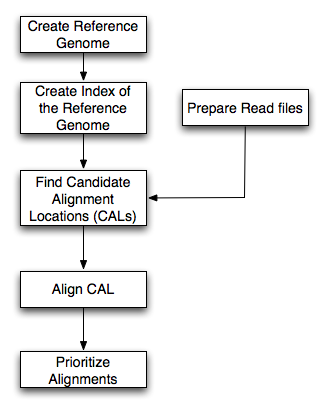
\includegraphics[scale=0.45]{figures/workflow.png} 
%
%\caption{\small Overall workflow for a mapping procedure using BFAST.  In this work, we focus on the step for finding Candidate Alignment Locations (CALs).  }
%  \label{fig:workflow-bfast} 
% \end{figure}
%
%
%\begin{table}
%\begin{tabular}{|c|c|c|c|} 
%  \hline 
% BFAST command & Description & Features for \\ 
%  &  &     Parallelism \\ \hline \hline
%\texttt{bfast fasta2brg} & creation of a ref. genome  &    multiple independent contigs \\ \hline 
%\texttt{solid2fastq}  &  preparation of short reads files &     multiple sequence reads files \\ \hline
%
%\texttt{bfast index} & creation of reference genome indexes& multi-threading and  \\
% &   & low memory option  \\  \hline
%\texttt{bfast match} & finding candidate alignment locations  &  multi-threading and  \\
%& &  parallel execution \\ \hline
%\texttt{bfast localalign} & alignment of each CAL  &   parallel execution \\  \hline
%\texttt{bfast postprocess} & prioritization of alignments  &  parallel execution \\ \hline
%
%
%\hline
%\end{tabular} \caption{Description of BFAST commands and features for parallel and multi-threading execution}
% \label{table:bfast-summary} 
%\end{table}
%

\section{Distributed Adaptive Runtime Environment}
\subsection{SAGA and BigJob abstraction}

To execute a scientific application using heterogeneous distributed computing resources, we develop the Distributed Adaptive Runtime Environment (DARE) framework\cite{dareurl}.  The framework is compose of an open source Web application framework, Pylons
and middleware of the application management system built upon SAGA an BigJob abstraction\cite{saga-ccgrid10,saga-royalsoc,saga-web,jha2009developing,ecmls10}.  This combination of the open source technology and the application management system enables us to develop a lightweight, extensible, full-fledged distributed computing science gateway quickly and effectively\cite{pylonsurl}. 

\subsection{Three DARE Tools}

\bibliographystyle{abbrv}
\bibliography{tg11}


\end{document}

